\documentclass[]{article}
\usepackage{tikz}
\usetikzlibrary{chains,fit, shadings, shadows, shapes, shapes.geometric, arrows, calc, positioning, shapes.geometric, arrows.meta, patterns, patterns.meta}

\tikzstyle{startstop} = [rectangle, rounded corners, minimum width=3cm, minimum height=1cm,text centered, draw=black, fill=red!30]
\tikzstyle{process} = [rectangle, minimum width=3cm, minimum height=1cm, text centered, draw=black, fill=orange!30]
\tikzstyle{decision} = [rectangle, minimum width=3cm, minimum height=1cm, text centered, draw=black, fill=green!30]
\tikzstyle{arrow} = [thick,->,>=stealth]
\usepackage{pgfplots}
\pgfplotsset{compat=1.16}
\usepackage{mathtools,amssymb}
%\input{Preamble}
%\input{(SpecialDistanceCourse}
%\input{FRAMES}
\begin{document}

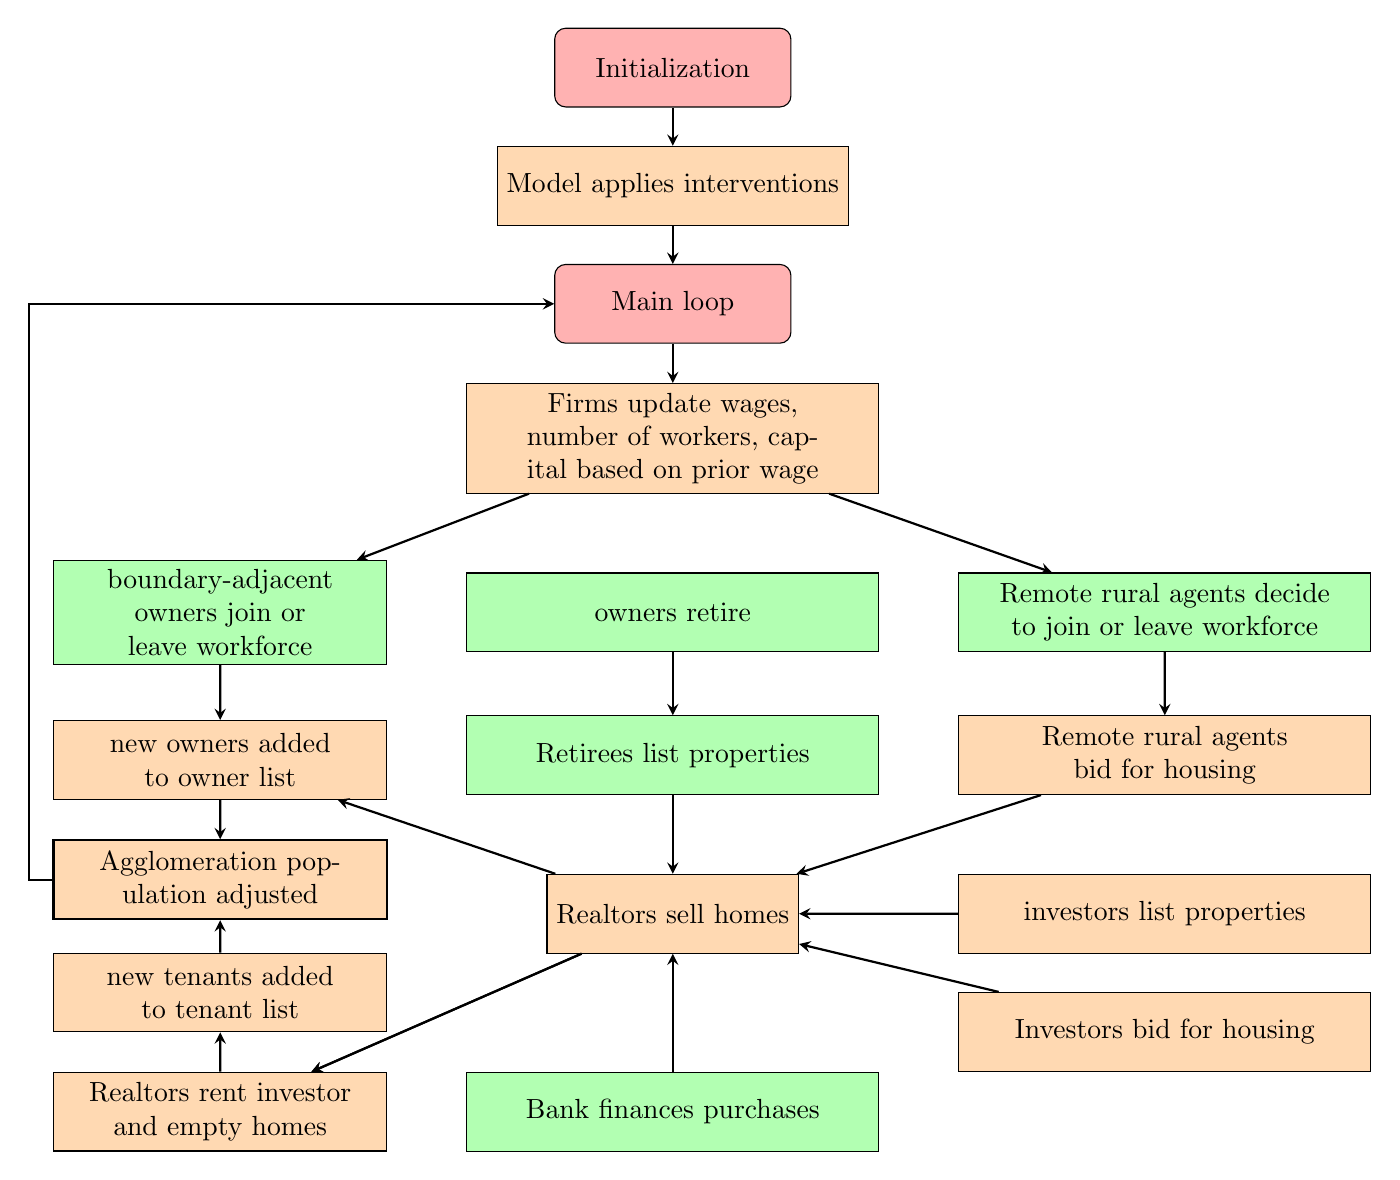
\begin{tikzpicture}[scale=.2,node distance=1.5cm]
\node (init) [startstop] {Initialization};
\node (interventions) [process, below of=init] {Model applies interventions};
% \node (record) [process, below of=interventions] {Record ownership share and reset counters};
\node (mainloop) [startstop, below of=interventions] {Main loop};
\node (firmupdate) [process, below=.5cm of mainloop, text width=5cm] {Firms update wages, number of workers, capital  based on prior wage};

    \draw [arrow] (init) -- (interventions);
    \draw [arrow] (interventions) -- (mainloop);
    \draw [arrow] (mainloop) -- (firmupdate);


\node (owners-retire) [decision, below=1cm of firmupdate, text width=5cm] {owners retire};
\node (rural-boundary) [decision, left= 1cm of  owners-retire,  text width=4cm] {boundary-adjacent owners  join or leave workforce};
\node (rural-remote) [decision,  right =1cm of owners-retire, text width=5cm] {Remote rural agents decide to join or leave workforce};


    \draw [arrow] (firmupdate) -- (rural-boundary);
    \draw [arrow] (firmupdate) -- (rural-remote);

\node (retired-list) [decision, below =.8cm of owners-retire, text width=5cm] {Retirees list properties};
  \draw [arrow] (owners-retire) -- (retired-list);



\node (Remote-bid) [process, right=1cm of retired-list, text width=5cm] {Remote rural agents bid for housing};
 \node (Invest-bid) [process, below=2.5cm of Remote-bid, text width=5cm] {Investors bid for housing};
    
%\node (invest-list) [process, green, below=6cm of rural-remote, text width=5cm] {investors list properties};land

\node (realtors_sell) [process, below = 1cm of retired-list ] {Realtors sell homes};
          \draw [arrow]  (retired-list) -- (realtors_sell);    
          \draw [arrow]  (Remote-bid) -- (realtors_sell);     
\node (invest-list) [process, below=1cm of Remote-bid, text width=5cm] {investors list properties};land
          \draw [arrow]  (invest-list) -- (realtors_sell);      
          \draw [arrow]  (Invest-bid) -- (realtors_sell);               
            
\node (bank) [decision, below =  of realtors_sell, text width=5cm] {Bank  finances purchases};
        \draw [arrow] (bank) -- (realtors_sell);

\node (realtors_rent) [process, left = 1cm of bank, text width=4cm] {Realtors rent investor and empty homes};
        \draw [arrow]  (realtors_sell) -- (realtors_rent)   ; 
        
\node (tenant-adjust) [process, above=.5cm of realtors_rent, text width=4cm] {new tenants added to tenant list};

        \draw [arrow]  (realtors_rent) -- (tenant-adjust)   ;

\node (owner-adjust) [process, below = .7cm of rural-boundary,  text width=4cm] {new owners added to owner list};
  \draw [arrow] (rural-boundary) -- (owner-adjust);
  
\node (agglom-adjust) [process, thick, below = .5cm of owner-adjust, text width=4cm] {Agglomeration population adjusted};


  \draw [arrow] (realtors_sell) -- (owner-adjust);
\draw [arrow] (rural-remote) -- (Remote-bid);
 \draw [arrow] (realtors_sell) -- (realtors_rent);
 \draw [arrow] (owner-adjust) -- (agglom-adjust);
\draw [arrow] (tenant-adjust) -- (agglom-adjust);

\draw [arrow] (agglom-adjust.west) -- ++(-1.5,0)  |- (mainloop); %-- ++(0,-.5) -- ++(7,0) |-
% % % Custom arrow path
% % \draw [arrow] ($(advance.south) + (0,-0.5)$) -- ++(0,-1) -- ($(mainloop.south) + (-2,-1)$) -- ($(mainloop.south) + (-2,0)$) -- (mainloop);

\end{tikzpicture}
\end{document}